\documentclass[a4paper, 12pt, final, garamond]{book}
\usepackage{cours-preambule}

\raggedbottom

\makeatletter
\renewcommand{\@chapapp}{M\'ecanique -- chapitre}
\makeatother

\begin{document}
\setcounter{chapter}{3}

\chapter{TD entra\^inement~: approche \'energ\'etique}

\section{Chute sur corde en escalade}
On étudie une grimpeuse qui chute. Une corde d'escalade de longueur $L_0$ peut,
en première approximation, être modélisée par un ressort de longueur à vide
$L_0$ et de raideur $k = \a/L_0$, avec $\a$ une caractéristique de la corde.

\begin{center}
    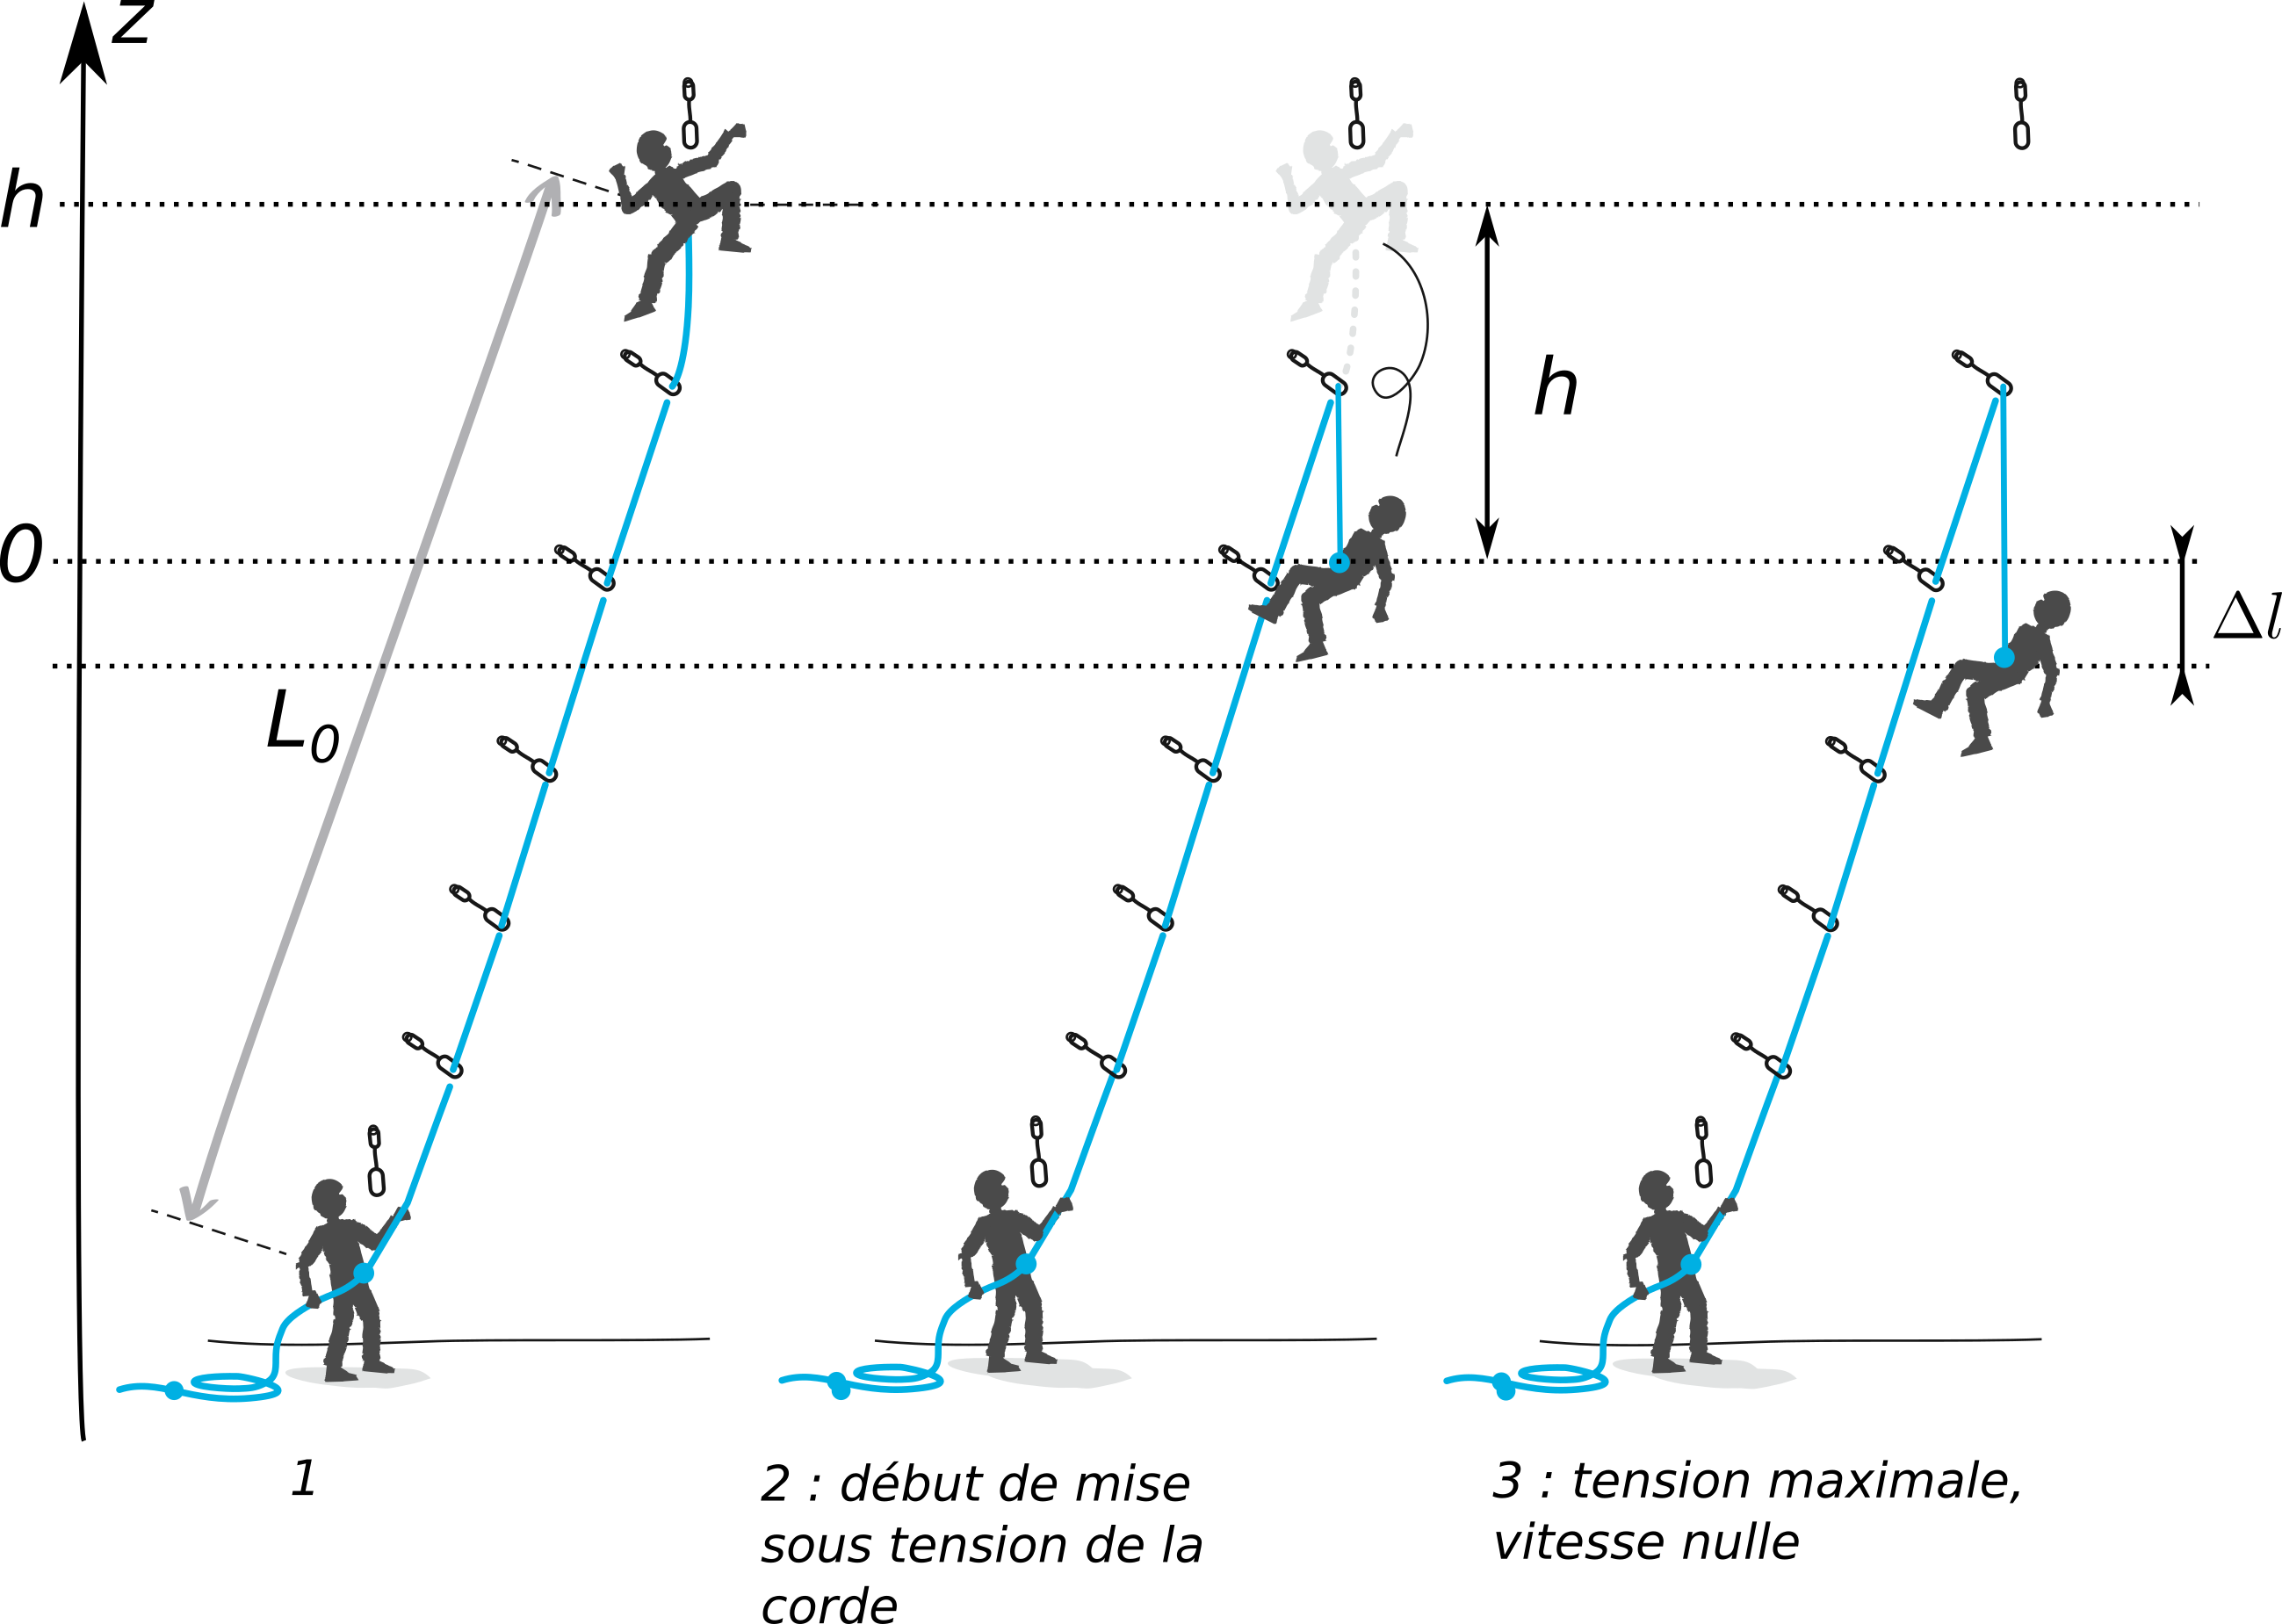
\includegraphics[width=.7\linewidth]{chute_escalade-plain}
\end{center}

La grimpeuse est en chute libre sur une hauteur $h$ pendant laquelle la corde
n'est pas sous tension. La corde passe ensuite sous tension, et la chute se
poursuit sur une hauteur $\D l$. La vitesse de la grimpeuse devient ainsi nulle
au bout d'une hauteur totale de chute $h+\D l$.

On prendra $g = \SI{10}{m.s^{-2}}$, $\a = \SI{5.0e4}{N}$ et une grimpeuse de
masse $m = \SI{50}{kg}$. \bigbreak

\begin{enumerate}
    \item À l'aide d'un bilan énergétique, donner l'expression de la vitesse
        maximale atteinte par la grimpeuse. Faire l'application numérique pour
        une hauteur de chute $h = \SI{5}{m}$.
    \item Toujours à l'aide d'une méthode énergétique, donner l'expression de
        l'allongement maximal $\D l$ de la corde. On supposera $\D l \ll h$ afin
        de simplifier le calcul.
    \item Donner enfin l'expression de la norme de la force maximal $F_{\max}$
        qu'exerce la corde sur la grimpeuse. On introduira le facteur de chute
        $f = h/L_0$.
    \item Au-delà d'une force de \SI{12}{kN}, les dommages sur le corps humain
        deviennent importants. Que vaut $F_{\max}$ pour une chute de $h =
        \SI{4}{m}$ sur une corde de longueur $L_0 = \SI{4}{m}$~? Conclure.
    \item Une chute d'un mètre arrêtée par une corde de \SI{50}{cm} est-elle
        plus ou moins dangereuse qu'une chute de \SI{4}{m} arrêtée par une corde
        de \SI{8}{m}~?
\end{enumerate}

\section{Pendule électrique}
On étudie un pendule constitué d'une boule de polystyrène expansé recouverte
d'une feuille d'aluminium, et suspendue à une potence par une fine tige de
longueur $R = \SI{10}{cm}$ dont nous négligerons la masse. La boule de masse $m
= \SI{20}{g}$ sera assimilée à un point matériel M.

\begin{minipage}{0.60\linewidth}
    Une boule identique est placée en A (voir schéma). Les deux boules sont
    chargées électriquement avec la même charge, et donc se repoussent. La force
    exercée par A sur M s'écrit
    \[\Ff_e = \frac{k}{\rm AM^3} \vv{\rm AM}
    \qavec
    k = \SI{4.4e-3}{N.m^2}\]
    \bigbreak
    \begin{enumerate}
        \item Exprimer la distance AM en fonction de $R$ et $\tt$.
        \item Montrer que la force $\Ff_e$ est conservative, et que son énergie
            potentielle s'exprime
            \[\Ec_{p,e}(\tt) = \frac{k}{R\sqrt{5-4\cos\tt}}\]
        \item Exprimer l'énergie potentielle totale $\Ec_p(\tt)$ de la boule M.
        \item Le tracé de l'énergie potentielle est proposé sur la figure 2. Déduire
            de ce graphe l'existence de positions d'équilibres, et indiquer leur
            nature.
        \item Discuter de la nature de la trajectoire de M suivant la valeur de son
            énergie mécanique.
    \end{enumerate}
\end{minipage}
\hfill
\begin{minipage}{0.35\linewidth}
    \begin{center}
        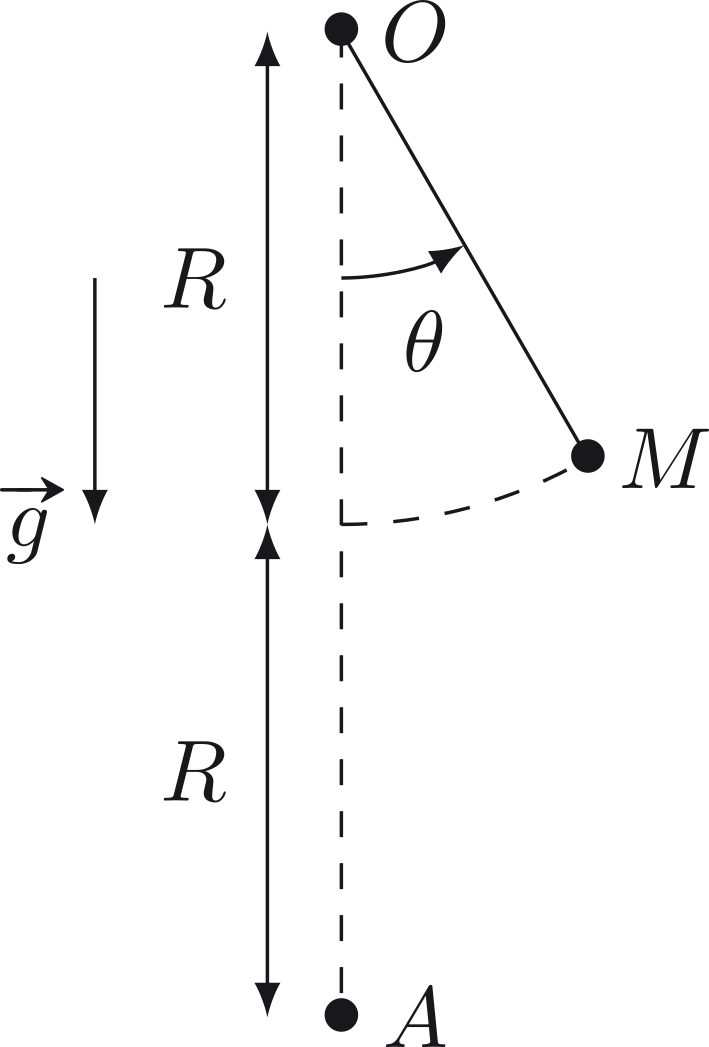
\includegraphics[height=4cm]{pendule_elec_sch-plain}
        \captionof{figure}{Dispositif}
    \end{center}
    \begin{center}
        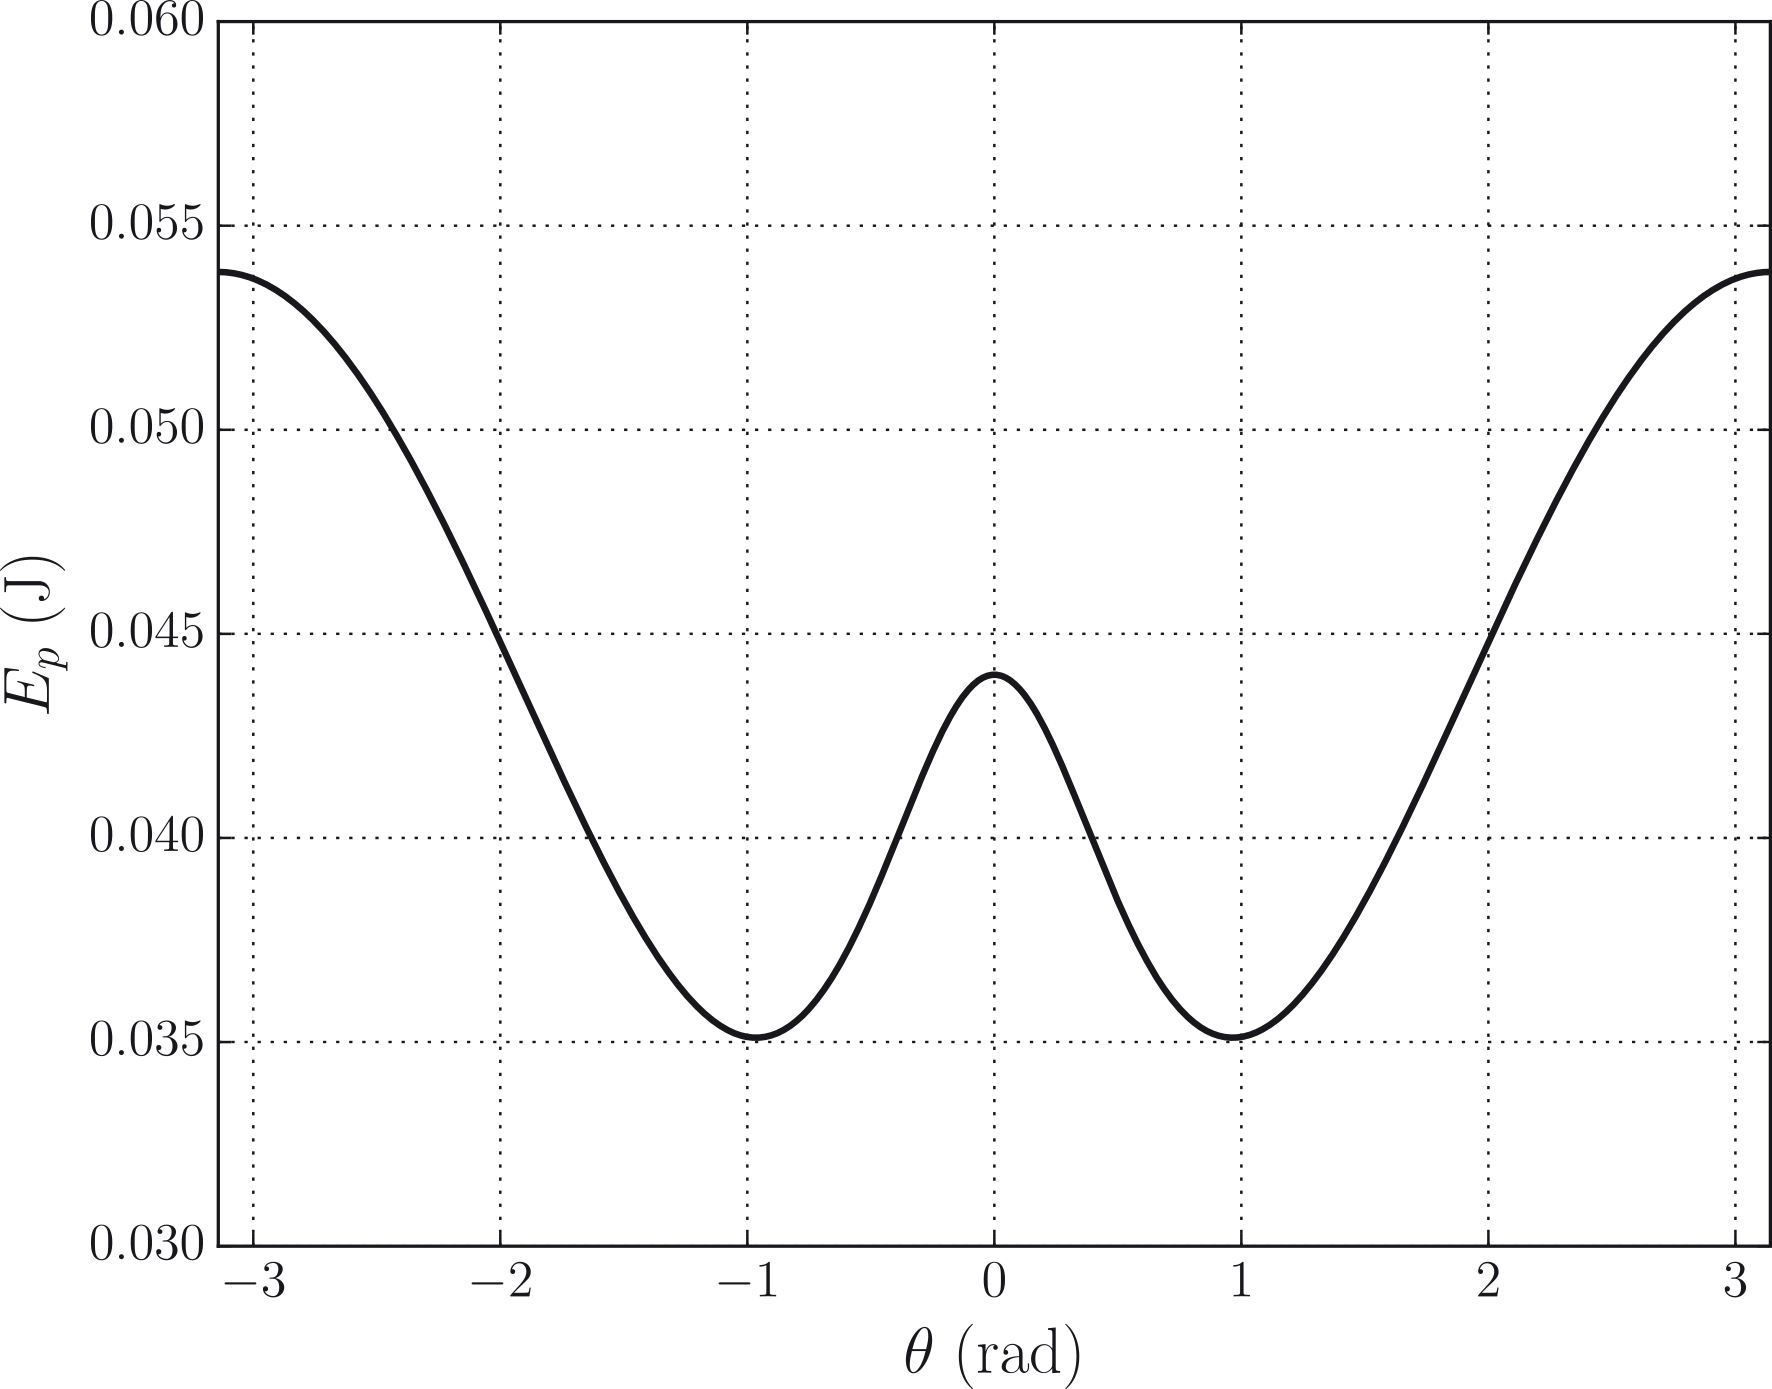
\includegraphics[width=\linewidth]{pendule_elec_ep-plain}
        \captionof{figure}{Courbe $\Ec_p(\tt)$}
    \end{center}
\end{minipage}


\section{Recul d'un canon}
On considère un canon (figure~\ref{fig:canon}) de masse $M = \SI{800}{kg}$. Lors
du tir horizontal d'un obus de masse $m = \SI{2.0}{kg}$ avec une vitesse
$\vfo=v_0\ux$ telle que $v_0 = \SI{600}{m.s^{-1}}$, le canon acquiert une
vitesse de recul $\vv{v_c} = -\frac{m}{M}\vfo$.

Pour limiter la course du canon, on utilise un ressort de raideur $k_1$, de
longueur à vide $L_0$ dont l'une des extrémités est fixe, et l'autre liée au
canon. Le déplacement a lieu suivant l'axe O$x$. Dans la suite, le canon est
assimilé à un point matériel, son centre de gravité G (figure~\ref{fig:rep}).

\begin{minipage}{0.40\linewidth}
    \begin{center}
        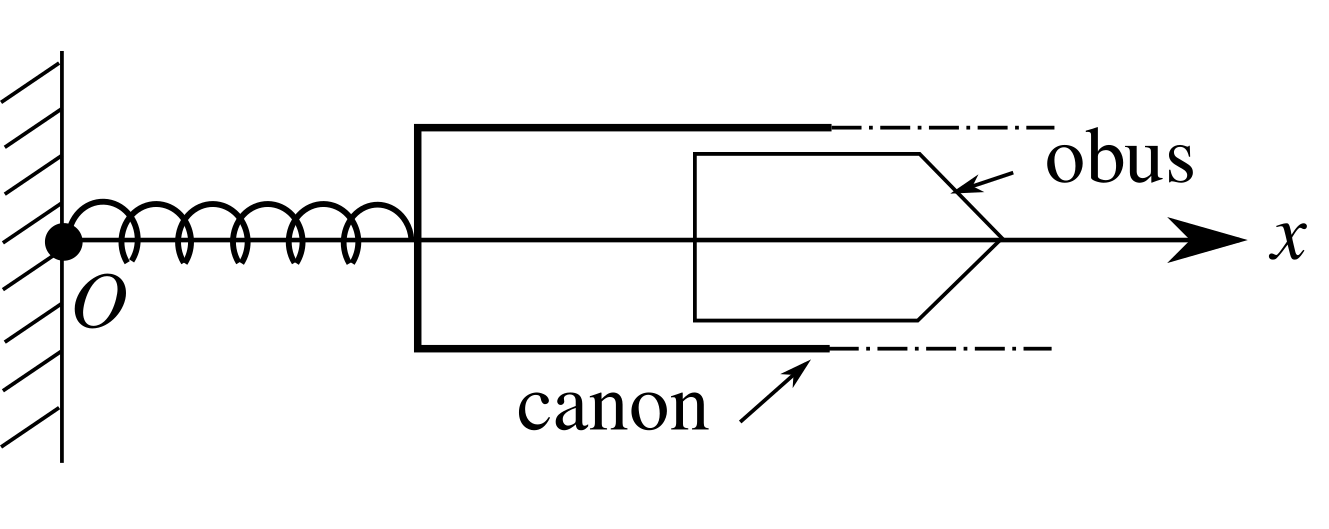
\includegraphics[height=3cm]{recul_canon_a-plain}
        \captionof{figure}{Canon}
        \label{fig:canon}
    \end{center}
\end{minipage}
\hfill
\begin{minipage}{0.23\linewidth}
    \begin{center}
        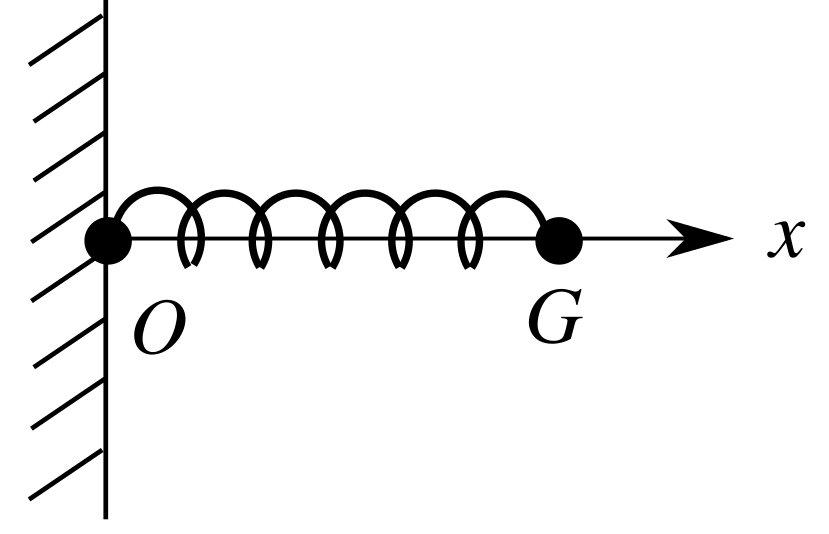
\includegraphics[height=3cm]{recul_canon_b-plain}
        \captionof{figure}{Repérage}
        \label{fig:rep}
    \end{center}
\end{minipage}
\hfill
\begin{minipage}{0.31\linewidth}
    \begin{center}
        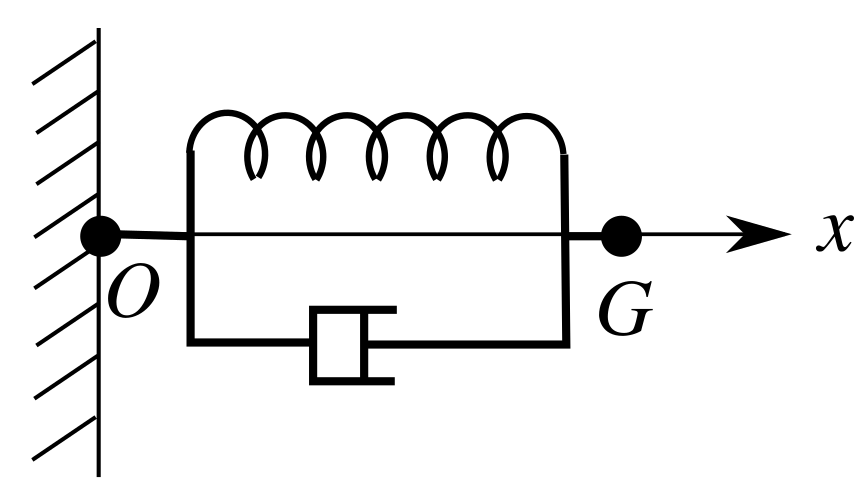
\includegraphics[height=3cm]{recul_canon_c-plain}
        \captionof{figure}{Amortisseur}
        \label{fig:amor}
    \end{center}
\end{minipage} \bigbreak

\begin{enumerate}
    \item Quelle est la longueur du ressort lorsque le canon est au repos~?
    \item En utilisant l'énergie mécanique, déterminer la distance de recul $d$.
        En déduire la raideur $k_1$ pour avoir un recul inférieur ou égal à $d$.
        Application numérique pour $d = \SI{1.0}{m}$.
    \item Retrouver la relation entre $k_1$ et $d$ en appliquant le PFD.
    \item Quel est l'inconvénient d'utiliser un ressort seul~?
\end{enumerate}
Pour pallier ce problème, on ajoute au système un dispositif amortisseur
(figure~\ref{fig:amor}), exerçant une force de frottement $\Ff = -\lb\vf$, $\vf$
étant la vitesse du canon.
\begin{enumerate}[resume]
    \item Le dispositif de freinage absorbe une fraction $\Ec_a = \SI{778}{J}$
        de l'énergie cinétique initiale. Calculer la nouvelle valeur $k_2$ de la
        constante de raideur du ressort avec les données numériques précédentes.
        Déterminer la pulsation propre $\w_0$ de l'oscillateur.
    \item Déterminer $\lb$ pour que le régime soit critique. Application
        numérique.
    \item Déterminer l'expression de l'élongation $x(t)$ du ressort, ainsi que
        celle de la vitesse $\xp(t)$. En déduire l'instant $t_m$ pour lequel le
        recul est maximal. Exprimer alors ce recul en fonction de $m$, $v_0$ et
        $\lb$. L'application numérique redonne-t-elle la valeur de $d$
        précédente~?
\end{enumerate}

\section{Positions d'équilibre d'un anneau sur un cercle}
\begin{minipage}{0.60\linewidth}
    Un anneau assimilable à un point matériel M de masse $m$ peut glisser sans
    frottement sur une glissière circulaire de rayon $R$ et de centre O.
    L'anneau est attaché à un ressort de raideur $k$ dont une extrémité est
    fixée à la glissière au point A. Sa position est repérée par l'angle $\tt$
    entre le rayon OM et l'axe horizontal (O$x$). Pour simplifier les calculs,
    on considérera que la longueur à vide $\ell_0$ du ressort est nulle.
\end{minipage}
\hfill
\begin{minipage}{0.35\linewidth}
    \begin{center}
        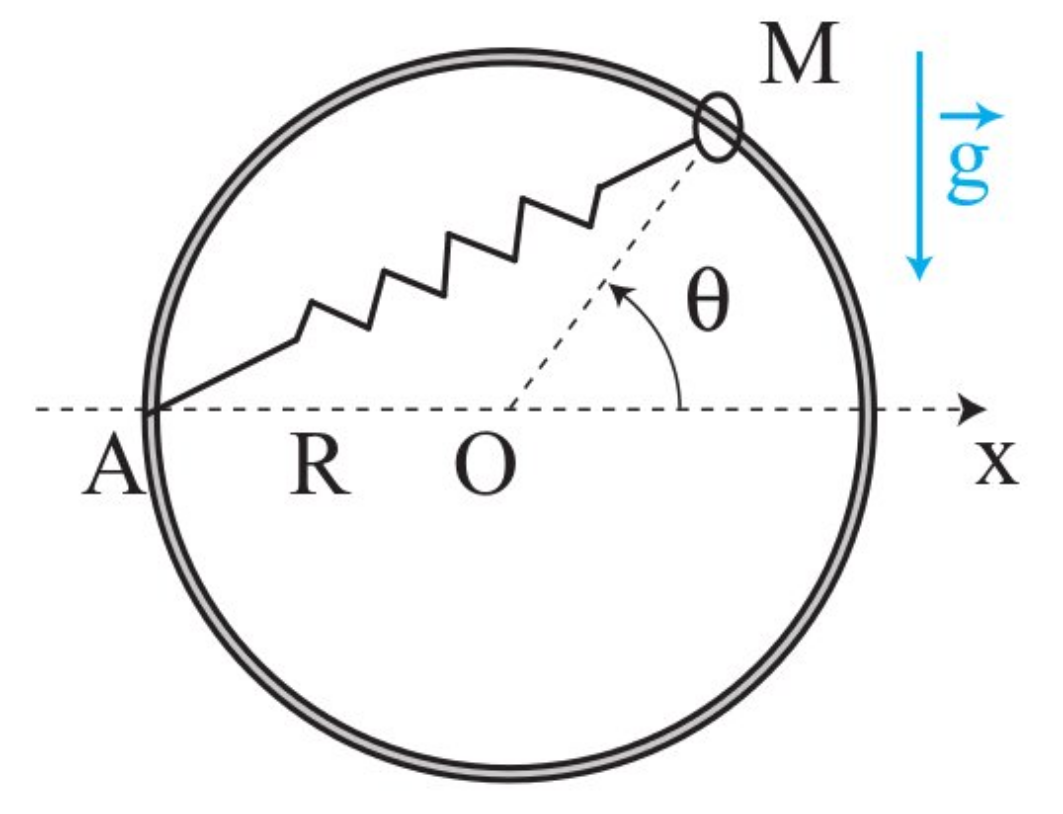
\includegraphics[width=.9\linewidth]{anneau_cercle_ressort-plain}
    \end{center}
\end{minipage}

\begin{enumerate}
    \item Montrer que la longueur $\ell$ s'exprime $\ell = R\sqrt{2(1+\cos\tt)}$.
    \item Exprimer l'énergie potentielle $\Ec_p$ du système constitué de
        l'anneau et du ressort en fonction de l'angle $\tt$.
    \item Déterminer les positions d'équilibre de l'anneau.
    \item Préciser si les positions d'équilibre obtenues sont stables.
\end{enumerate}

\section{Oscillateur de \textsc{Landau}}

L'oscillateur de \textsc{Landau} est un modèle théorique permettant de modéliser
efficacement des systèmes physiques pour lesquelles des faibles non-linéarités
sont à prendre en compte. Il s'agit d'une approximation un peu plus précise que
celle de l'oscillateur harmonique pour étudier le comportement de systèmes au
voisinage de leur position d'équilibre. \bigbreak

\begin{minipage}{0.70\linewidth}
    Un exemple de système modèle permettant de réaliser un oscillateur de Landau
    est un petit anneau, assimilé à un point matériel M de masse $m$, astreint à
    se déplacer sans frottement le long d'une tige rectiligne horizontale
    choisie comme axe (O$x$). Cet anneau est relié à un ressort, de longueur à
    vide $\ell_0$ et de raideur $k$, dont l'autre extrémité est fixée en A. La
    distance de A à la tige est notée ${\rm AO} = a$.
\end{minipage}
\hfill
\begin{minipage}{0.25\linewidth}
    \begin{center}
        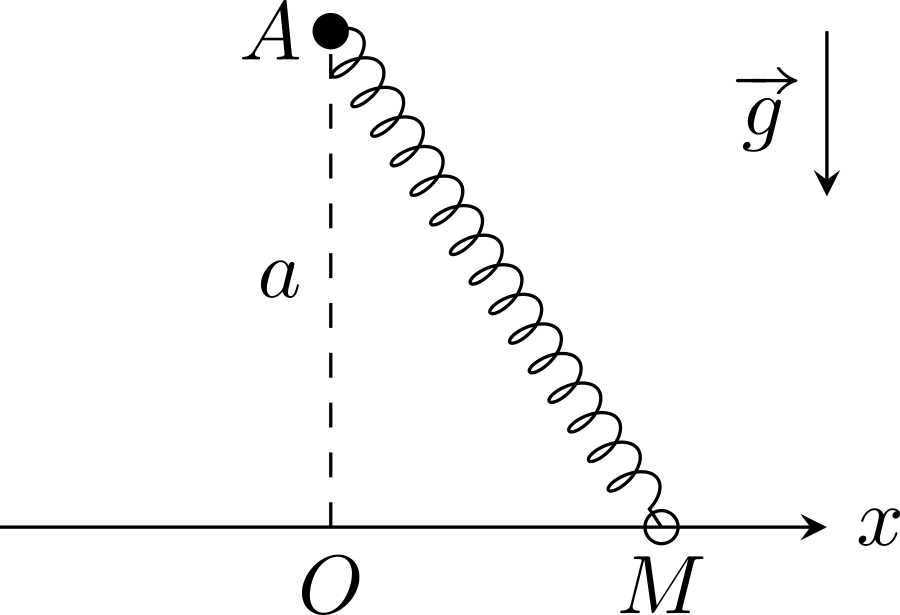
\includegraphics[width=\linewidth]{landeau_sch-plain}
    \end{center}
\end{minipage} \bigbreak

\begin{enumerate}
    \item Exprimer l'énergie potentielle totale $\Ec_p(x)$.
    \item La courbe d'énergie potentielle est représentée ci-dessous pour quatre
        valeurs de $a$~: $a_1 = \ell_0/10$, $a_2 = \ell_0/3$, $a_3 = \ell_0$ et
        $a_4 = 3\ell_0$. En raisonnement qualitativement sur les positions
        d'équilibre, attribuer chaque courbe à la valeur de $a$ qui lui
        correspond.
    \item Pour chaque valeur de $a$, analyser le mouvement possible de l'anneau
        en fonction des conditions initiales.
    \item Pour les valeurs de $a$ précédentes, l'anneau est lâché avec les mêmes
        conditions initiales. Sa vitesse et sa position sont enregistrées au
        cours du temps, ce qui donne les trajectoires de phase de la figure
        ci-dessous. Déterminer la condition initiale et affecter chaque
        trajectoire de phase à la valeur de $a$ qui lui correspond.
\end{enumerate} \bigbreak

\begin{minipage}{0.45\linewidth}
    \begin{center}
        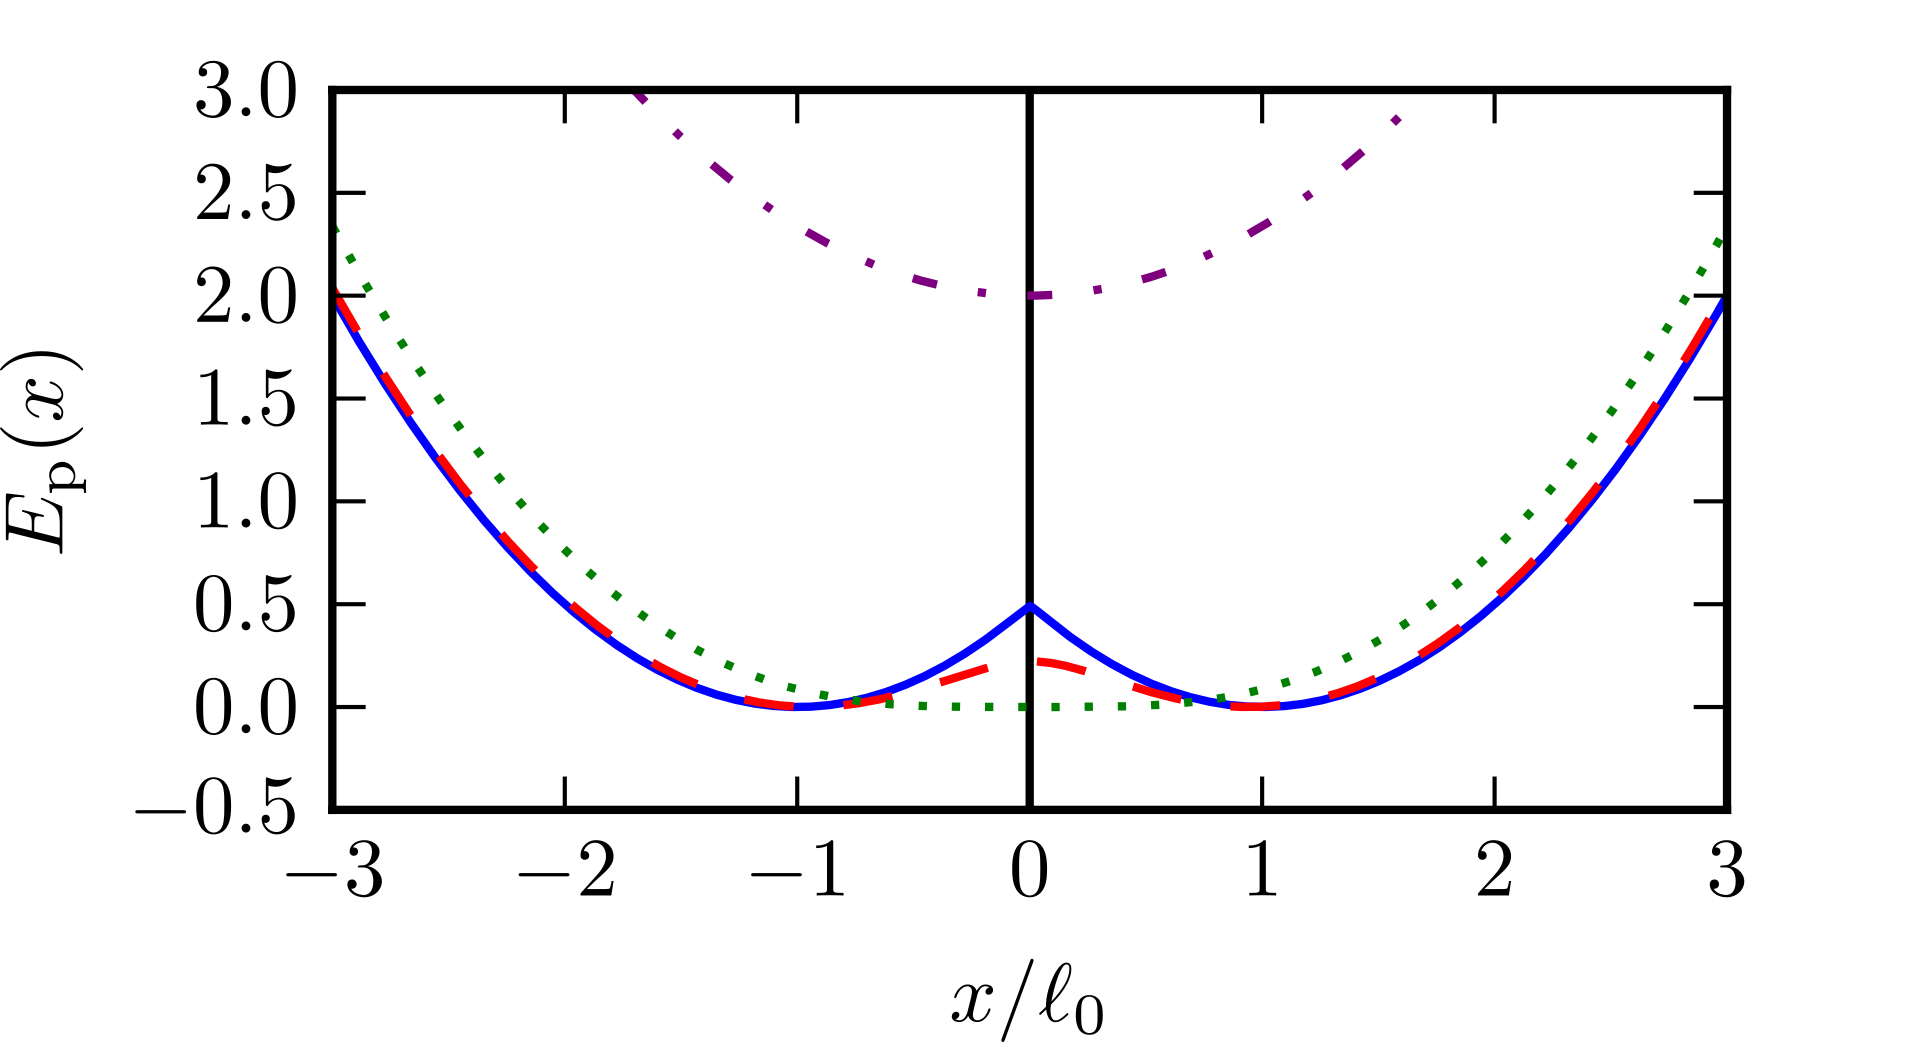
\includegraphics[width=\linewidth]{landeau_ep-plain}
    \end{center}
\end{minipage}
\hfill
\begin{minipage}{0.45\linewidth}
    \begin{center}
        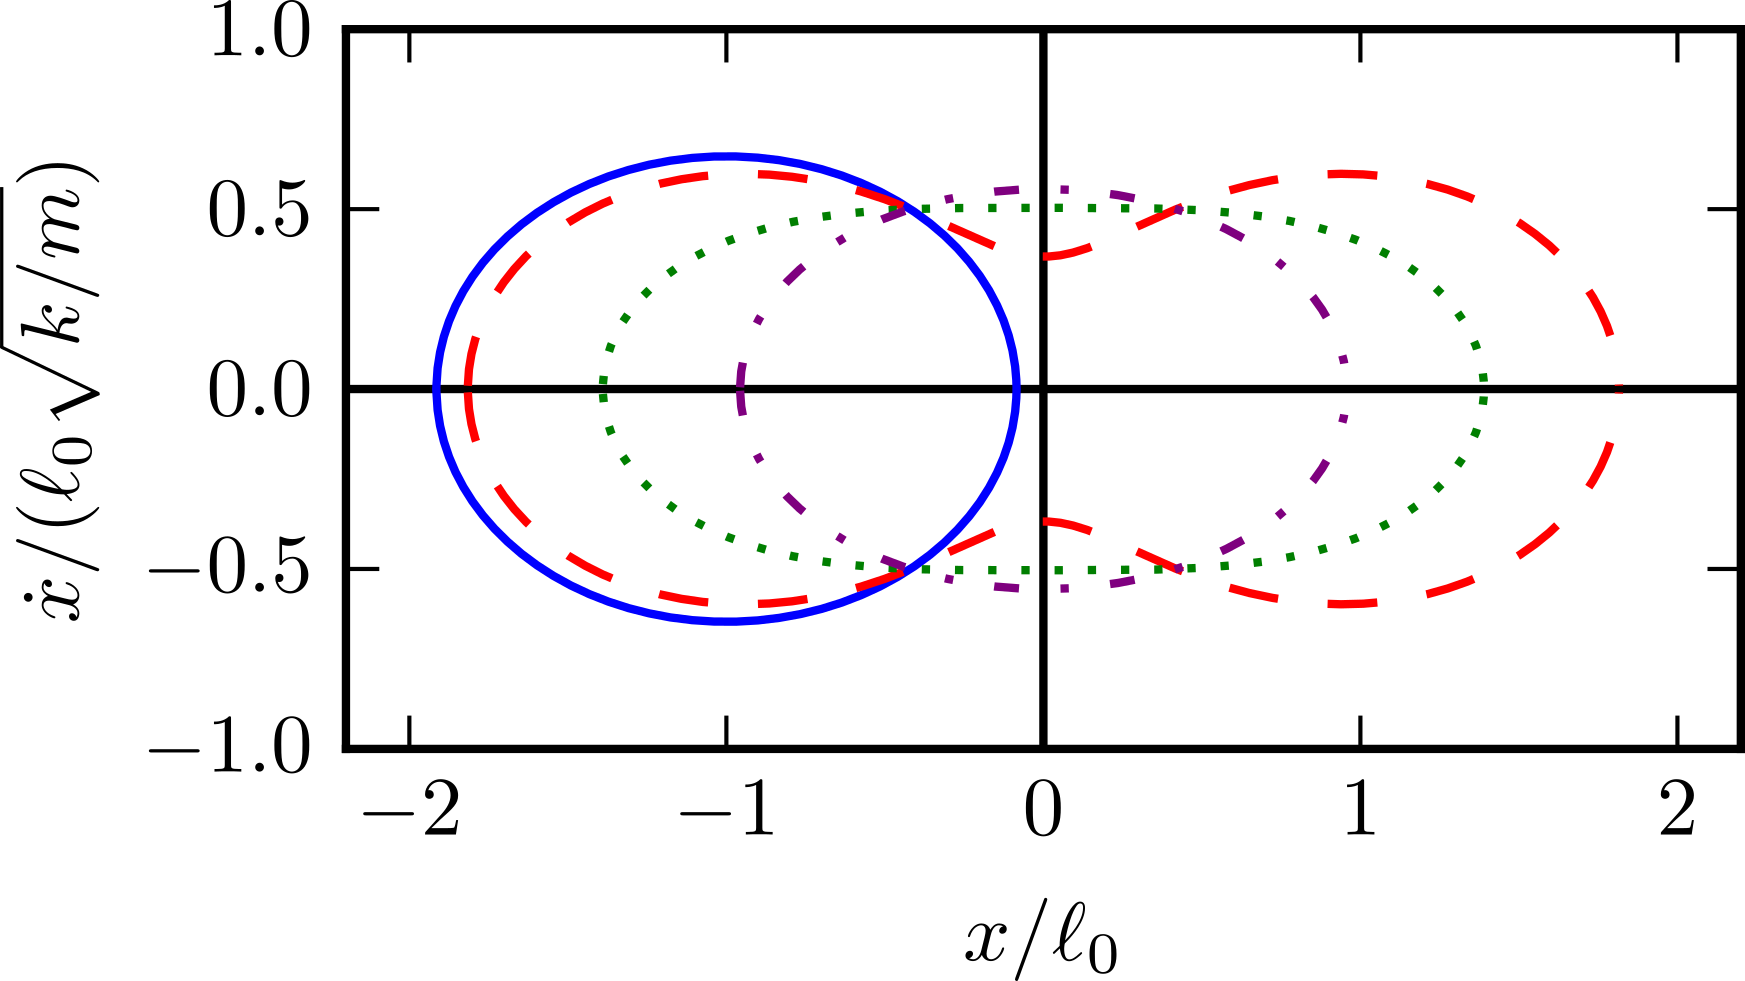
\includegraphics[width=\linewidth]{landeau_xp-plain}
    \end{center}
\end{minipage}


\end{document}
